\documentclass[letterpaper]{article}
\usepackage{alltt}
\usepackage{graphicx}
\usepackage{xspace}
\usepackage{color}
\usepackage{amsmath}
\definecolor{linkcolor}{RGB}{16,65,69}

\newcommand{\ttt}[1]{\texttt{#1}}
\newcommand{\projname}{\ttt{bt}\xspace}

\newenvironment{monospace}{\begin{quote}\begin{alltt}}{\end{alltt}\end{quote}}

\author{Joe Colosimo \\ \small{colosimo@mit.edu} \\ Group 6}
\date{\today}

\usepackage[colorlinks=true, linkcolor=linkcolor]{hyperref}
\title{\projname{} - A Realtime Beat Tracker \\ Final Report}
\begin{document}

\maketitle

\section{Primary Objective}
    \projname is a live beat tracker --- a device that reads a stream of music
    and, in realtime, makes a guess at its tempo.  

    Beat analysis is an important field of audio signal processing.  It's used
    in a variety of applications in the music universe.  For example, DJ
    software finds the tempo and beat locations of the tracks in the user's
    library beforehand in order to make synchronizing two playing tracks a
    straightforward process.  It's also used in audio-controlled lighting to
    generate complex displays that react to music.

    Most of the time, beat analysis is done before its information is actually
    needed.  As a result, these preprocessing algorithms (there are numerous)
    can be very accurate.


\section{Background}

    Realtime tempo estimation of a live stream is a difficult problem to solve,
    especially compared to a pre-processing-based approach.  In this case,
    we're looking not only to accurately identify a best estimate for the
    tempo, but also to converge on that estimate as quickly as possible.

    One algorithm involves trying to classify portions of a music stream as
    ``beats" and then tries to match those beats against one of many possible
    tempos, eventually narrowing in on a most likely candidate.

    This includes creating a series of phase-locking metronomes, each running
    at a different tempo, and trying to match detected beats to subdivision of
    each metronome.


\section{Why Dedicated Hardware?}

    This algorithm is more of an entertaining novelty than anything else;
    nobody would actually use it in a real product.  But it does offer some
    interesting ideas with respect to parallelism.  Namely, dedicated hardware
    offers the ability to instantiate, for example, 60 or 70 different
    metronomes with very precise timing, all running independently of one
    another.  This would not be possible using conventional CPU architecture --
    most threaded models lose precision after just a few metronomes.
    Furthermore, realtime beat classification is a challenging algorithm to
    implement on most CPUs, even though there are often plenty of clock cycles
    between audio samples.  Although this project does not use a
    frequency-aware beat classification algorithm, it one were to switch to it,
    one would surely desire dedicated hardware for taking large FFTs.


\section{High Level Design}
    
    Figure~\ref{fig:architecture} illustrates the overall
    architecture of the system.

    \begin{figure}
        \centering
        %\includegraphics{fig/architecture.pdf}
        \caption{\projname algorithm architecture}
        \label{fig:architecture}
    \end{figure}

    The system starts off by instantiating metronomes with a wide range of
    tempos.  The number of metronomes is limited by the resource constraints of
    the system.  They all wait for the beat classifier to seed them with an
    initial guess at a beat, at which point they start running.  After this
    initialization phase, the metronomes keep time, each at their own tempo,
    and when the beat classifier detects a beat in the audio, it delivers a
    message to all of the metronomes stating the likelihood that the event it
    just saw was a beat.  The metronomes then all adjust their phase linearly
    with the probability that the beat classifier thought it was correct and
    report their current phase difference to the metronome bank controller.

    In this manner, metronomes whose tempo is different from the stream's real
    tempo will consistently report large phase errors, while those closer to
    the real tempo will report smaller phase errors.  We can then use these
    results to generate a probability distribution for the actual tempo.
    Optionally, after a period of convergence, we can ``zoom in" on the
    possible tempos, trying smaller and smaller increments around the most
    likely tempo until we converge on a reasonable result.  This project does
    not include that features because enough metronomes were instantiated to
    fit a large range of tempos with per-BPM precision.


\section{Testing}


\section{Microarchitecture}
    \subsection{Top Level}

        The top level module of \projname{} handles inter-module communication as
        well as sample injection and hardware output.

        \subsection{Interface to Hardware Architecture}

        The hardware produces audio samples and then requires a handshake to read
        the sample.  From the hardware side, the \ttt{sample\_injector} module
        provides the following signals:

        \begin{center}
        \begin{tabular}{|r|l|}
            \hline
            \ttt{sample} & \ttt{out std\_logic\_vector(13 downto 0)} \\ \hline
            \ttt{sample\_rdy} & \ttt{out std\_logic} \\ \hline
            \ttt{sample\_rd} & \ttt{in std\_logic} \\ \hline
        \end{tabular}
        \end{center}

        \projname{} therefore waits for input \ttt{sample\_rdy} to go high, at
        which point it captures \ttt{sample} and asserts \ttt{sample\_rd = '1'} for
        one clock cycle.  It enqueues the sample to the beat classifier's input
        FIFO through its \ttt{InjectSample} method.

        \subsubsection{Output}
            
        The output of the top module is a (wide) parallel bus that is an array of
        the attempted tempos and their respective likelihoods.  The hardware
        architecture takes care of splitting this bus up into bytes for output via
        serial.

        \subsubsection{Submodules}

        There is a single beat classifier, a vector of metronomes, and a single
        metronome bank controller.  As discussed later, the top level takes care of
        tasks such as iterating a command, such as \ttt{SetMetronomeTempo} from the
        metronome bank controller to all of the metronomes.


    \subsection{Beat Classifier}

        The beat classifier handles the process of receiving injected audio samples
        and determining when the audio stream has likely produced a beat.


        \subsubsection{Operation}
            
        The beat classification algorithm essentially compares the local energy of
        a small sample window to the average energy of a much larger window.  If
        there is significant deviation of the local energy from the average energy
        (either positive or negative), then the beat classifier reports that it saw
        a beat.

        It runs a round of this every time it receives a sample via its
        \ttt{InjectSample} method, described below.  When a new sample has been
        presented, it computes this instantaneous energy of the sample, by squaring
        it and accumulates this to the \ttt{LocalEnergy} register.  When $N_L$ of
        such samples are accumulated, we are ready to compare the local energy with
        the average energy, which is held in the \ttt{AverageEnergy} register.  If
        the local energy is different from the average energy by a factor $F$, we
        report a beat by setting a \ttt{Maybe} register valid as described in
        Section~\ref{sec:bc:metif}.

        We then update the average energy register using a simple EWMA scheme:
        \begin{equation}
            \textrm{\ttt{AverageEnergy}} = \alpha \textrm{\ttt{AverageEnergy}} +
                            (1-\alpha) \textrm{\ttt{LocalEnergy}}
        \end{equation}

        where $\alpha$ is some number less than 1 and represents the degree of
        decay.  Another way to handle the \ttt{AverageEnergy} would be to instead
        keep a buffer of local energies and take an arithmetic average.  This also
        allows us to compute the variance of the local energies, which would allow
        us to approximate $F$ far better than if it were constant.

        
        \subsubsection{Tunable Parameters}

        There are a few parameters here that can be fine-tuned.

        $N_L$ basically asks "how many samples corresponds to local energy?".  If
        it's too small, we may not get a good enough estimate of the signal energy
        at any given point, but if it's too large, then we could be including a
        beat with non-beat portion of the spectrum.  Experiments suggest that $N_L
        \approx 1000$ works well.

        $F$ determines just how different the local energy has to be from the
        average energy for a beat to be considered.  In practice, if we were to
        think of the ratio of local energy to average energy, $F$ usually works
        well at about 1.2 or 1.3.  However, this can vary by genre.  This is why I
        would eventually like to be able to compute the variance of local energies
        to determine a best fit for F.

        $\alpha$ determines the decay rate of the average energy.  A low value of
        $\alpha$ indicates that we want to consider recent energies much, much more
        than older energies.  However, in this case, $\alpha$ should be fairly
        high, around 0.6 or 0.7.  If $\alpha$ is too high, however, we could run
        into issues where the overall energy of the track has changed but the
        average energy doesn't quite catch up to reflect that.  $\alpha$ will be
        represented as a \ttt{FixedPoint} fraction.


        \subsubsection{Interface to Top-Level Injector: \ttt{InjectSample}}

        The module has a very small FIFO through which input samples come in on.
        The method \ttt{InjectSample} simply enqueues a sample for processing.
            

        \subsubsection{Interface to the Metronomes: \ttt{SawBeat}}
        \label{sec:bc:metif}

        For a given input sample, if the beat classifier has detected a beat,
        it delivers a message to all of the metronomes.  To do this, it
        maintains a register of type \ttt{Maybe\#(BeatLikelihood)} that it
        updates on each clock cycle where a valid value indicates that a beat
        was discovered.  The \ttt{BeatLikelihood} type is a way for the
        classifier to indicate to the metronomes just how likely it thought
        what it just saw was a beat.  This allows the metronomes to adjust
        their phase accordingly, as is discussed later in this document.

        To read this register, the beat classifier module provides a method
        called \ttt{SawBeat} that returns its contents.  The top level module
        calls this method on every clock cycle and when the value returned is
        valid, calls the \ttt{InjectBeat} method of each metronome with the
        likelihood as an argument.


    \subsection{Metronome}

        The metronome keeps time to a given tempo.  Essentially, it's a fancy
        counter that's not unlike something that one would use as the phase ramp
        input to a lookup table for a DDS.

        \subsubsection{Operation}

        The metronome uses a fixed point representation where the integer part is
        only 2 bits and the decimal part is much larger (as large as possible while
        still fitting within the resource constraints).  The integer part
        represents sixteenth notes.  When it rolls over from 3 to 0, a quarter note
        has occurred.


        \subsubsection{Setting the Tempo: \ttt{SetTempo}}

        This sets the amount that the counter is incremented by with each clock
        cycle.  In the language of DDSes, this is the slope of the phase ramp.


        \subsubsection{Starting the Metronome: \ttt{Start}}

        This method resets all of the counters to 0 and enables counting.


        \subsubsection{Injecting a Beat: \ttt{InjectBeat}}
        
        When the beat classifier detects a beat, it indicates this to all of the
        metronomes.  The metronome responds by adjusting its counter's phase to be
        closest to the nearest sixteenth note according to the \ttt{BeatLikelihood}
        value.  It also returns the phase offset that it had to apply to achieve
        this back to the top level module (which goes on to deliver this
        information to the metronome bank controller).

        The base implementation will simply just set the phase to the nearest
        sixteenth note, but the more advanced implementation will do so linearly
        according to the \ttt{BeatLikelihood} value.  So, for example, if the value
        was 0.5, the phase will be set to halfway between its current value and the
        nearest sixteenth note.


    \subsection{Metronome Bank Controller}

        The metronome bank controller collects all of the metronome phase
        differences and uses that to generate the parallel output stream, but also
        to set the tempos of the individual metronomes.

        For each metronome, it keeps track of an EWMA'd running average for the
        phase error.  Each time the metronome reports a phase error, the controller
        computes the new average phase error as $\alpha \textrm{\ttt{AvgPhaseErr}}
        + (1-\alpha) \textrm{\ttt{PhaseError}}$.  In this case $\alpha=0.5$.

        The parallel output stream is simply generated by shoving all the metronome
        tempos and their respective average phase errors (with 16 bits of precision)
        into a parallel bus.

        The other major thing that the controller does is with each update of the
        average phase error, is to compute their gradient.  If the maximum and
        minimum differ by a large enough factor, the bank controller will ``zoom
        in" to a new set of tempos based on where the phase error is minimal.
        Experimentation showed that it works best to close in on the convergence by
        a factor of two.  That is, if the previous range spanned 100~BPM, the next
        range should span 50~BPM, etc.


\section{Evaluation}
    I've been designing this project very close to hardware -- I do live
    hardware testing just as much as I do simulation testing.  So I've been
    conscious of device timing and area constraints the entire time.

    I've been testing with just 3 metronomes. The synthesis results that the
    logic usage is absolutely tiny:

\begin{monospace}
Device utilization summary:
---------------------------

Selected Device : 3s700anfgg484-4 

 Number of Slices:           422  out of   5888     7%
 Number of Slice Flip Flops: 440  out of  11776     3%
 Number of 4 input LUTs:     769  out of  11776     6%
    Number used as logic:    729
    Number used as RAMs:      40
 Number of IOs:               36
 Number of bonded IOBs:       25  out of    372     6%
 Number of MULT18X18SIOs:      1  out of     20     5%
 Number of GCLKs:              2  out of     24     8%
 Number of DCMs:               1  out of      8    12%
\end{monospace}

Examining the timing analysis report, the critical path is through the beat
classifier, with the majority of the time is from the energy calculation path.

Let's take a look if we bump the number of metronomes up to 63:
\begin{monospace}
Device utilization summary:
---------------------------

Selected Device : 3s700anfgg484-4 

 Number of Slices:           2138  out of   5888    36%
 Number of Slice Flip Flops: 2806  out of  11776    23%
 Number of 4 input LUTs:     3934  out of  11776    33%
 Number of IOs:                36
 Number of bonded IOBs:        25  out of    372     6%
 Number of BRAMs:               1  out of     20     5%
 Number of MULT18X18SIOs:       1  out of     20     5%
 Number of GCLKs:               2  out of     24     8%
 Number of DCMs:                1  out of      8    12%
\end{monospace}

The critical path is once again through the beat classifier to the new beat
injector.

Right now, attempts at building with 120 metronomes fails to meet timing but I
bet I could probably get it to synthesize properly with some work.  This would
eliminate the need for field narrowing.


\section{Design Exploration --- Thoughts for the Future}
    \subsection{Variance-Sensitive Beat Classifier}
        
        If we store about 1 second worth of energies, we can perform the following
        linear regression to determine a good fit for the ratio of the current
        instantaneous energy to the last second of average energy in order to
        detect a beat.  Thus, we're looking for:

        \begin{align}
            \frac{e}{\mu_E} \geq 1.5142857 - 0.0025714 \sigma^2_E
        \end{align}

        where $\mu_E$ is the average energy, $e$ is the current instantaneous
        energy, and $\sigma^2$ is the variance of the last second's worth of
        energies.  More specifically:

        \begin{align}
            \mu_E &= \frac{1}{n} \sum_{i=0}^{n-1} e_i \\
            \sigma^2_E &= \mu_{E^2} - (\mu_E)^2
        \end{align}

        We can rearrange these equations to be more suitable for implementation in
        a digital system:

        \begin{align}
            e \geq & 1.5142857 \mu_E  - 0.0025714 \sigma^2_E \mu_E \\
            \geq & 1.5142857 \mu_E
                    - 0.0025714 (\mu_{E^2} - (\mu_E)^2) \mu_E \\
            \geq & 1.5142857 \mu_E
                    - 0.0025714 \mu_E \mu_{E^2} 
                    + 0.0025714 (\mu_E)^3 \\
            \geq & 1.5142857 \frac{1}{n} \sum_{i=0}^{n-1} e_i \\
                & - 0.0025714 \left[
                                    \left(\frac{1}{n} \sum_{i=0}^{n-1} (e_i)^2\right) +
                                    \left(
                                        \left(\frac{1}{n} \sum_{i=0}^{n-1} e_i\right) \cdot
                                        \left(\frac{1}{n} \sum_{i=0}^{n-1} e_i\right)
                                    \right)
                                \right] \cdot
                                \left(\frac{1}{n} \sum_{i=0}^{n-1} e_i\right)
        \end{align}


        So, if we keep a shift register of the last $n$ energies, as well as the
        last $n$ energies squared, as well as a running sum of those two, then we
        can simply subtract the oldest value and add the newest value with each new
        input energy.  This allows us to quickly compute variance with just one
        extra cycle.  From there, we can use Bluespec's \ttt{FixedPoint} library to
        compute the value of $e$ in two more cycles (I'm limiting one
        multiplication per cycle due to resource constraints on the FPGA.  We then
        can compare $e$ to the current instantaneous energy to see if a beat event
        occurred or not.

        The current design does this in 4 linearly-pipelined stages.

        I'm still working on getting the algorithm to function correctly.  There's
        an error in the mathematical implementation.  I was surprised (and happy)
        to see that I can actually perform all these calculations with full
        numerical precision, though I have a mechanism in place to truncate results
        at certain stages to reduce bit-width growth.


\end{document}
